
\section{Results}

\begin{frame}{Outline of simulation study}

\begin{itemize}
  \item Let two agents learn on two different state spaces, ''hand'' \& ''sum''
  \item Both spaces have the same amount of decks in play
  \item Agents start of \textit{exactly} the same, same q-learning algorithm,  etc. 
  \item For each state/action, track the avg. return (and values of $q$). 
  \item Agents get to play $10^7$ episodes of blackjack. 
\end{itemize}

\end{frame}

\begin{frame}{Avg. return}

\begin{figure}
\begin{tabular}{cc}
\centering
 \begin{subfigure}[b]{0.48\textwidth}
  	 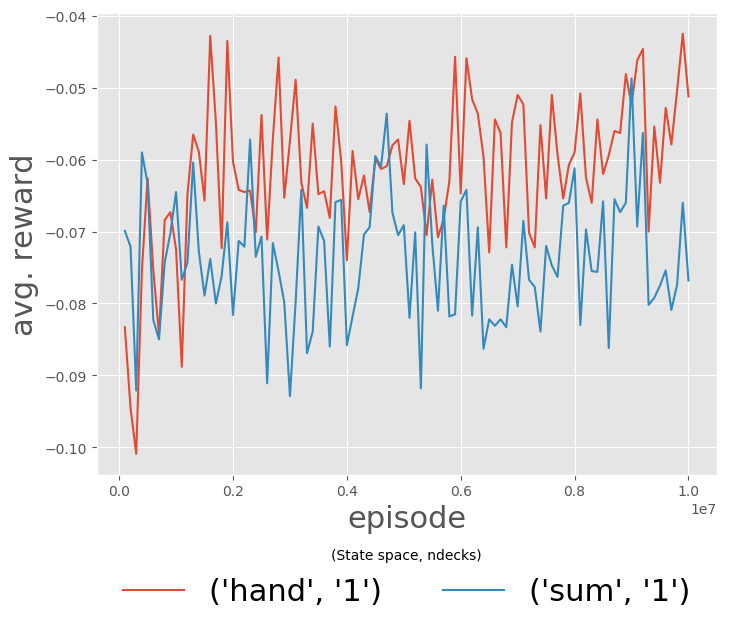
\includegraphics[width=\textwidth]{../report/figures/avgReturnEp_ndeck1.png}
   % .: 0x0 pixel, 0dpi, 0.00x0.00 cm, bb=
   \caption{Avg. return with 1 deck}
 \end{subfigure}
 &
 \begin{subfigure}[b]{0.48\textwidth}
  	 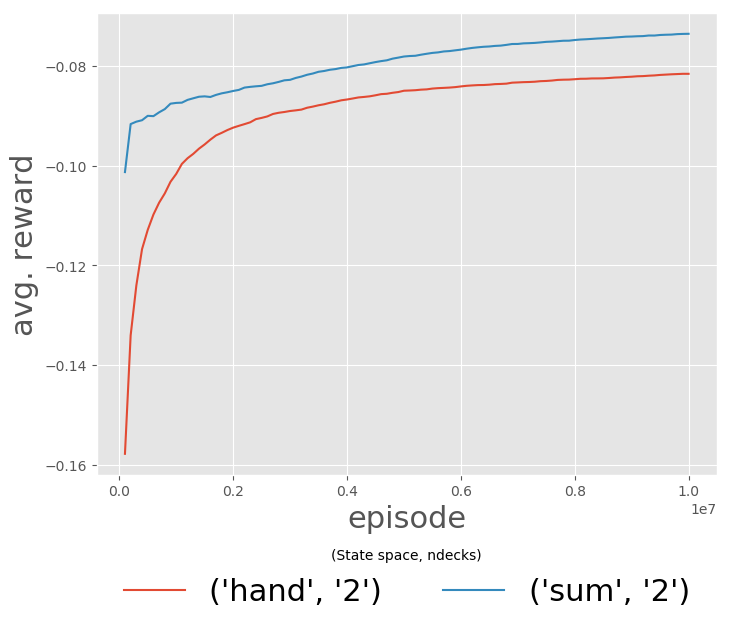
\includegraphics[width=\textwidth]{../report/figures/avgReturnEp_ndeck2.png}
   % .: 0x0 pixel, 0dpi, 0.00x0.00 cm, bb=
   \caption{Avg. return with 2 decks}
 \end{subfigure}
\end{tabular}
\end{figure}

\end{frame}

\begin{frame}{Number of visited states, learning time}
\begin{table}[h!]
\centering
 \begin{tabular}{c|cc|cc}
  \# decks & $\#S_{hand}$ & $t_{hand}$ & $\#S_{sum}$ &  $t_{sum}$  \\
  \hline 
  $1$ & $7651$ & $1510.681$ & $641$ & $1003.765$ \\
  $2$ & $38266$ & $1565.314$ & $677$ & $1079.656$ \\
  $8$ & $70034$ & $1606.944$ & $695$ & $1079.626$ \\
  $\inf$ & $70307$ & $1636.044$ & $671$ & $1097.971$ 
 \end{tabular} 
 \caption{The number of explored states $\#S$ and the training time $t$ (seconds) for a given number of decks in play and its respective state space.\label{tab:state_visited}}
\end{table}
\end{frame}

\section{Summary}

\begin{frame}{Discussion}

\begin{itemize}
 \item Q-learning on two representations of the state space of blackjack
 \item Performance? Simpler representation is better (Cardinality of the larger representation is immense!)
 \item Longer training time $\rightarrow$ results might be different 
 \item Extensions: Several agents, memory to the agent $\rightarrow$ counting cards? 
\end{itemize}

\end{frame}